\subsection{Backscattering}

Poniamo le nostre lamine a \SI{150}{\degree} (il valore più grande sulla scala graduata) per verificare la presenza di backscattering. Usiamo 2 lamine attaccate per essere sicuri che nessuna particella attraversi il bersaglio. Questo accorgimento ci permette di evitare che delle particelle $\alpha$ entrino nel rivelatore dopo essere rimbalzate sulle pareti. Abbiamo controllato che questa ipotesi sia sensata contando le particelle che attraversano 2 lamine dello stesso materiale (e spessore) a \SI{0}{\degree}.

Facendo misure con \SI{40}{\micro m} di oro non abbiamo osservato nessun evento nei \SI{1406}s\,$\approx$\,\SI{23}{minuti} della misura. La situazione è diversa per \SI{16}{\micro m} di alluminio: abbiamo un rate di \SI{0.57(8)}{s^{-1}}.
Questo risultato però non è il nostro fondo perché nelle misure a \SI{150}{\degree} sarà rappresentato da quelle particelle $\alpha$ che, rimbalzando sulle pareti, arrivano nel fotodiodo. Sappiamo anche che il fondo maggiore è rappresentato dalle particelle che arrivano al rivelatore dopo aver rimbalzato sui supporti di plastica delle lamine.

Abbiamo quantificato quest'ultimo effetto ponendo un supporto senza lamina al centro della camera e misurando il rate a \SI{150}{\degree}. Otteniamo $R_{\text{buco}}=\SI{3.9(6)e-4}{s^{-1}}$.
Siccome in presenza dell'alluminio le particelle che raggiungono la parete opposta alla sorgente sono ancora meno che nella situazione precedente, possiamo affermare che il fondo è minore di quello misurato. Ci aspettiamo che il rate di fondo sia trascurabilmente minore di $R_{\text{buco}}$ sia per motivi geometrici che dinamici. La particella $\alpha$ in questione dovrebbe colpire un piccolo rivelatore rimbalzando in una grande camera a vuoto e la sezione d'urto differenziale Rutherford decresce molto velocemente per angoli inferiori a \SI{10}{\degree}. Inoltre, nei rimbalzi ad angolo maggiore, la perdita di energia è più elevata. Questi meccanismi sfavoriscono diffusioni multiple all'interno della camera.

Di seguito riportiamo i risultati delle nostre misure di backscattering:
\begin{align*}
R_{\text{oro}} &= \SI{1.3(2)e-3}{s^{-1}} \\
R_{\text{alluminio}} &= \SI{5.4(6)e-4}{s^{-1}} \\
R_{\text{fondo}} \simeq R_{\text{buco}} &= \SI{3.9(6)e-4}{s^{-1}} \\
\text{differenza oro-fondo} &= \SI{5.9(4)}{\sigma} \\
\text{differenza alluminio-fondo} &= \SI{2.6(11)}{\sigma} \\
\end{align*}

Possiamo affermare in modo indiscutibile l'esistenza del backscattering nel caso dell'oro, ma non possiamo fare altrettanto con l'alluminio, almeno in questa misura.
Per poter osservare un indiscutibile backscattering anche con l'alluminio, abbiamo posto 2 ampi dissipatori per transistor in prossimità del fotodiodo e della sorgente a \SI{150}{\degree}.
Le dimensioni dei dissipatori impediscono alle particelle $\alpha$ di attraversarli e sono colpiti dalla quasi totalità del fascio, restituendoci una misura praticamente priva di fondo.
L'autopassivazione dell'alluminio crea uno strato di ossido spesso da 1 a \SI5{nm}, che viene portato a 50--\SI{200}{nm} con processi industriali.%
\footnote{\url{http://www.valocchi.eu/logistica/alluminio.htm}}
Data la sottigliezza di tale spessore, consideriamo trascurabile la variazione del rate dovuta a questo strato che è dovuta alla diversa densità dell'ossido e alla presenza dei nuclei di ossigeno.
Abbiamo ottenuto \SI{54(7)}{eventi} in circa \SI{6.5}{ore}.

\paragraph{Perdita di energia per scattering all'indietro} Dalla \autoref{eq:tout}, per uno scattering a \SI{150}{\degree} ci aspetteremmo che le particelle $\alpha$ arrivino al rivelatore con un energia pari rispettivamente al $\sim$ 45\% e 92\% dell'energia cinetica iniziale per diffusione su alluminio e oro. Bisogna tener conto del fatto che essendo le lamine spesse (rispetto alla lunghezza di radiazione) lo scattering Rutherford può avvenire in profondità per cui l'energia osservata non è quella attesa per il singolo urto ma sostanzialmente minore a causa dell'energia persa nel mezzo per interazione con gli elettroni. Gli spettri osservati per gli eventi di backscattering su oro e alluminio sono mostrati in \autoref{fig:backscattering}.
La bassa statistica non permette di concludere molto. Gli spettri sembrano piccare entrambi alla stessa energia: questo può essere qualitativamente spiegato dal fatto che sebbene le particelle $\alpha$ dopo lo scattering su oro abbiano circa il doppio dell'energia rispetto all'urto su alluminio, la lamina di oro usata è più spessa e l'energia persa in unità di lunghezza maggiore rispetto all'alluminio.

\begin{figure}[h]
	\centering
	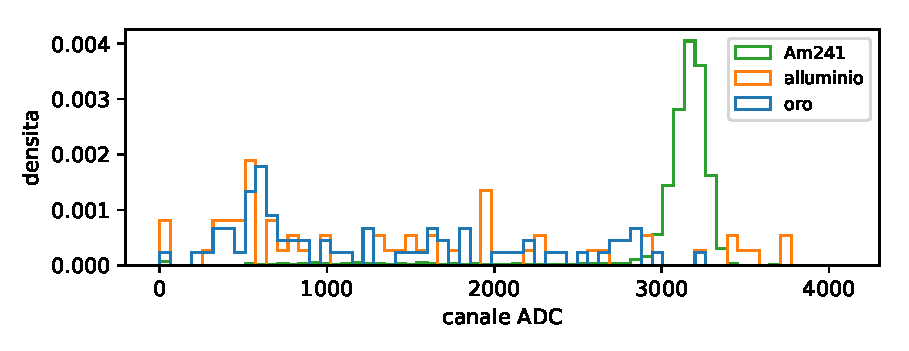
\includegraphics[width=30 em]{immagini/backscattering}
	\caption{Spettro delle particelle diffuse all'indietro per oro e alluminio. In verde lo spettro degli $\alpha$ provenienti dalla nostra sorgente.}
	\label{fig:backscattering}
\end{figure}